\documentclass{standalone}
\begin{document} 

\subsection{Aufgabe 4.5}
% ozi
\begin{itemize}
	\item[a)] Mittelpunkt kann man durch: 
	$[(1,1,1)^T + (2\lambda,\lambda,0)]^T]/2$ rechnen und $M=\vec{x}^T=(\frac{2\lambda+1}{2},\frac{\lambda+1}{2},\frac{1}{2})$ \\
	\item[b)] Die senkrechte Ebene rechnet man mit Formel: $ E=\vec{v} * (\vec{x}-\vec{p}) = 0 $\\
	Also, unsre Ebene heißt:\\
	$E=(2\lambda,\lambda,0)*[\vec{x}*(\frac{2\lambda+1}{2},\frac{\lambda+1}{2},\frac{1}{2})]$
	\item[c)] Die Teilaufgaben bei c) beschreibt alle Ebenen. Das bedeutet, dass das Z-Achse Komponente von jedem Ebene keine Bedeutung hat. Einfach die Linie bei der x-y Ebene rechnen und dann mit dem gesamten Z-Achse die Antwort(Ebene) bauen.\\
	\item[d)] Kugel;Punkt. Laut das Kugelformel:\\
	$(x-\frac{2\lambda+1}{2})^2 + (y -\frac{\lambda+1}{2})^2) + (z-\frac{1}{2}) \le (\frac{|\vec{x}|}{2})^2$\\
	\item[e)]Die Schnitt der Kugel mit der x-y Achsen ist einfach ein Kreis:\\
	$(x-\frac{2\lambda+1}{2})^2 + (y -\frac{\lambda+1}{2})^2)=(\frac{|\vec{x}|}{2})^2$
\end{itemize}

\subsection{Aufgabe 4.6}
%ozi
$\frac{a}{b} \textless \frac{c}{d} \leftrightarrow ad \textless bc$ Wir können das beweisen indem wir die nachgefragte Ungleichung in zwei teilen betrachten. Zuerst: \\
$\frac{a}{b} \textless \frac{a+c}{b+d} \equiv a(b+d) \textless b(a+c)$
$\equiv ab+ad \textless ab+bc$ Wir subtrahieren die Term "ab" zu beiden Seiten. Dann folgt $ ad \textless bc$ also, es ist wahr.\\

Der zweiten Teil:\\
$\frac{a+c}{b+d} \textless \frac{c}{d}$
$d(a+c) \textless c(b+d)$
$\equiv da+dc \textless bc+dc $ Wir subtrahieren die Term "dc" zu beiden Seiten. Dann folgt $ ad \textless bc$ also, es ist wahr.\\

\subsection{Aufgabe 4.7}
%ozi
Wenn man x mit y addiert bekommt man: $x+y=a$;\\
Wenn man x mit y subtrahiert bekommt man: $x-y=b$, also:\\
$|a+b|+|a-b| \ge |a|+|b| \equiv $\\
$|2x|+|2y| \ge |x+y|+|x-y| \equiv$\\
$(|2x|+|2y|)^2 \ge (|x+y|+|x-y|)^2 \equiv$ ... \\
$ 8xy \ge 0$\\
Das ist wahr.

\subsection{Aufgabe 4.8}
%ozi
\begin{itemize}
	\item[a)] Graphic: 
	\begin{figure}[htbp]
		\centering
		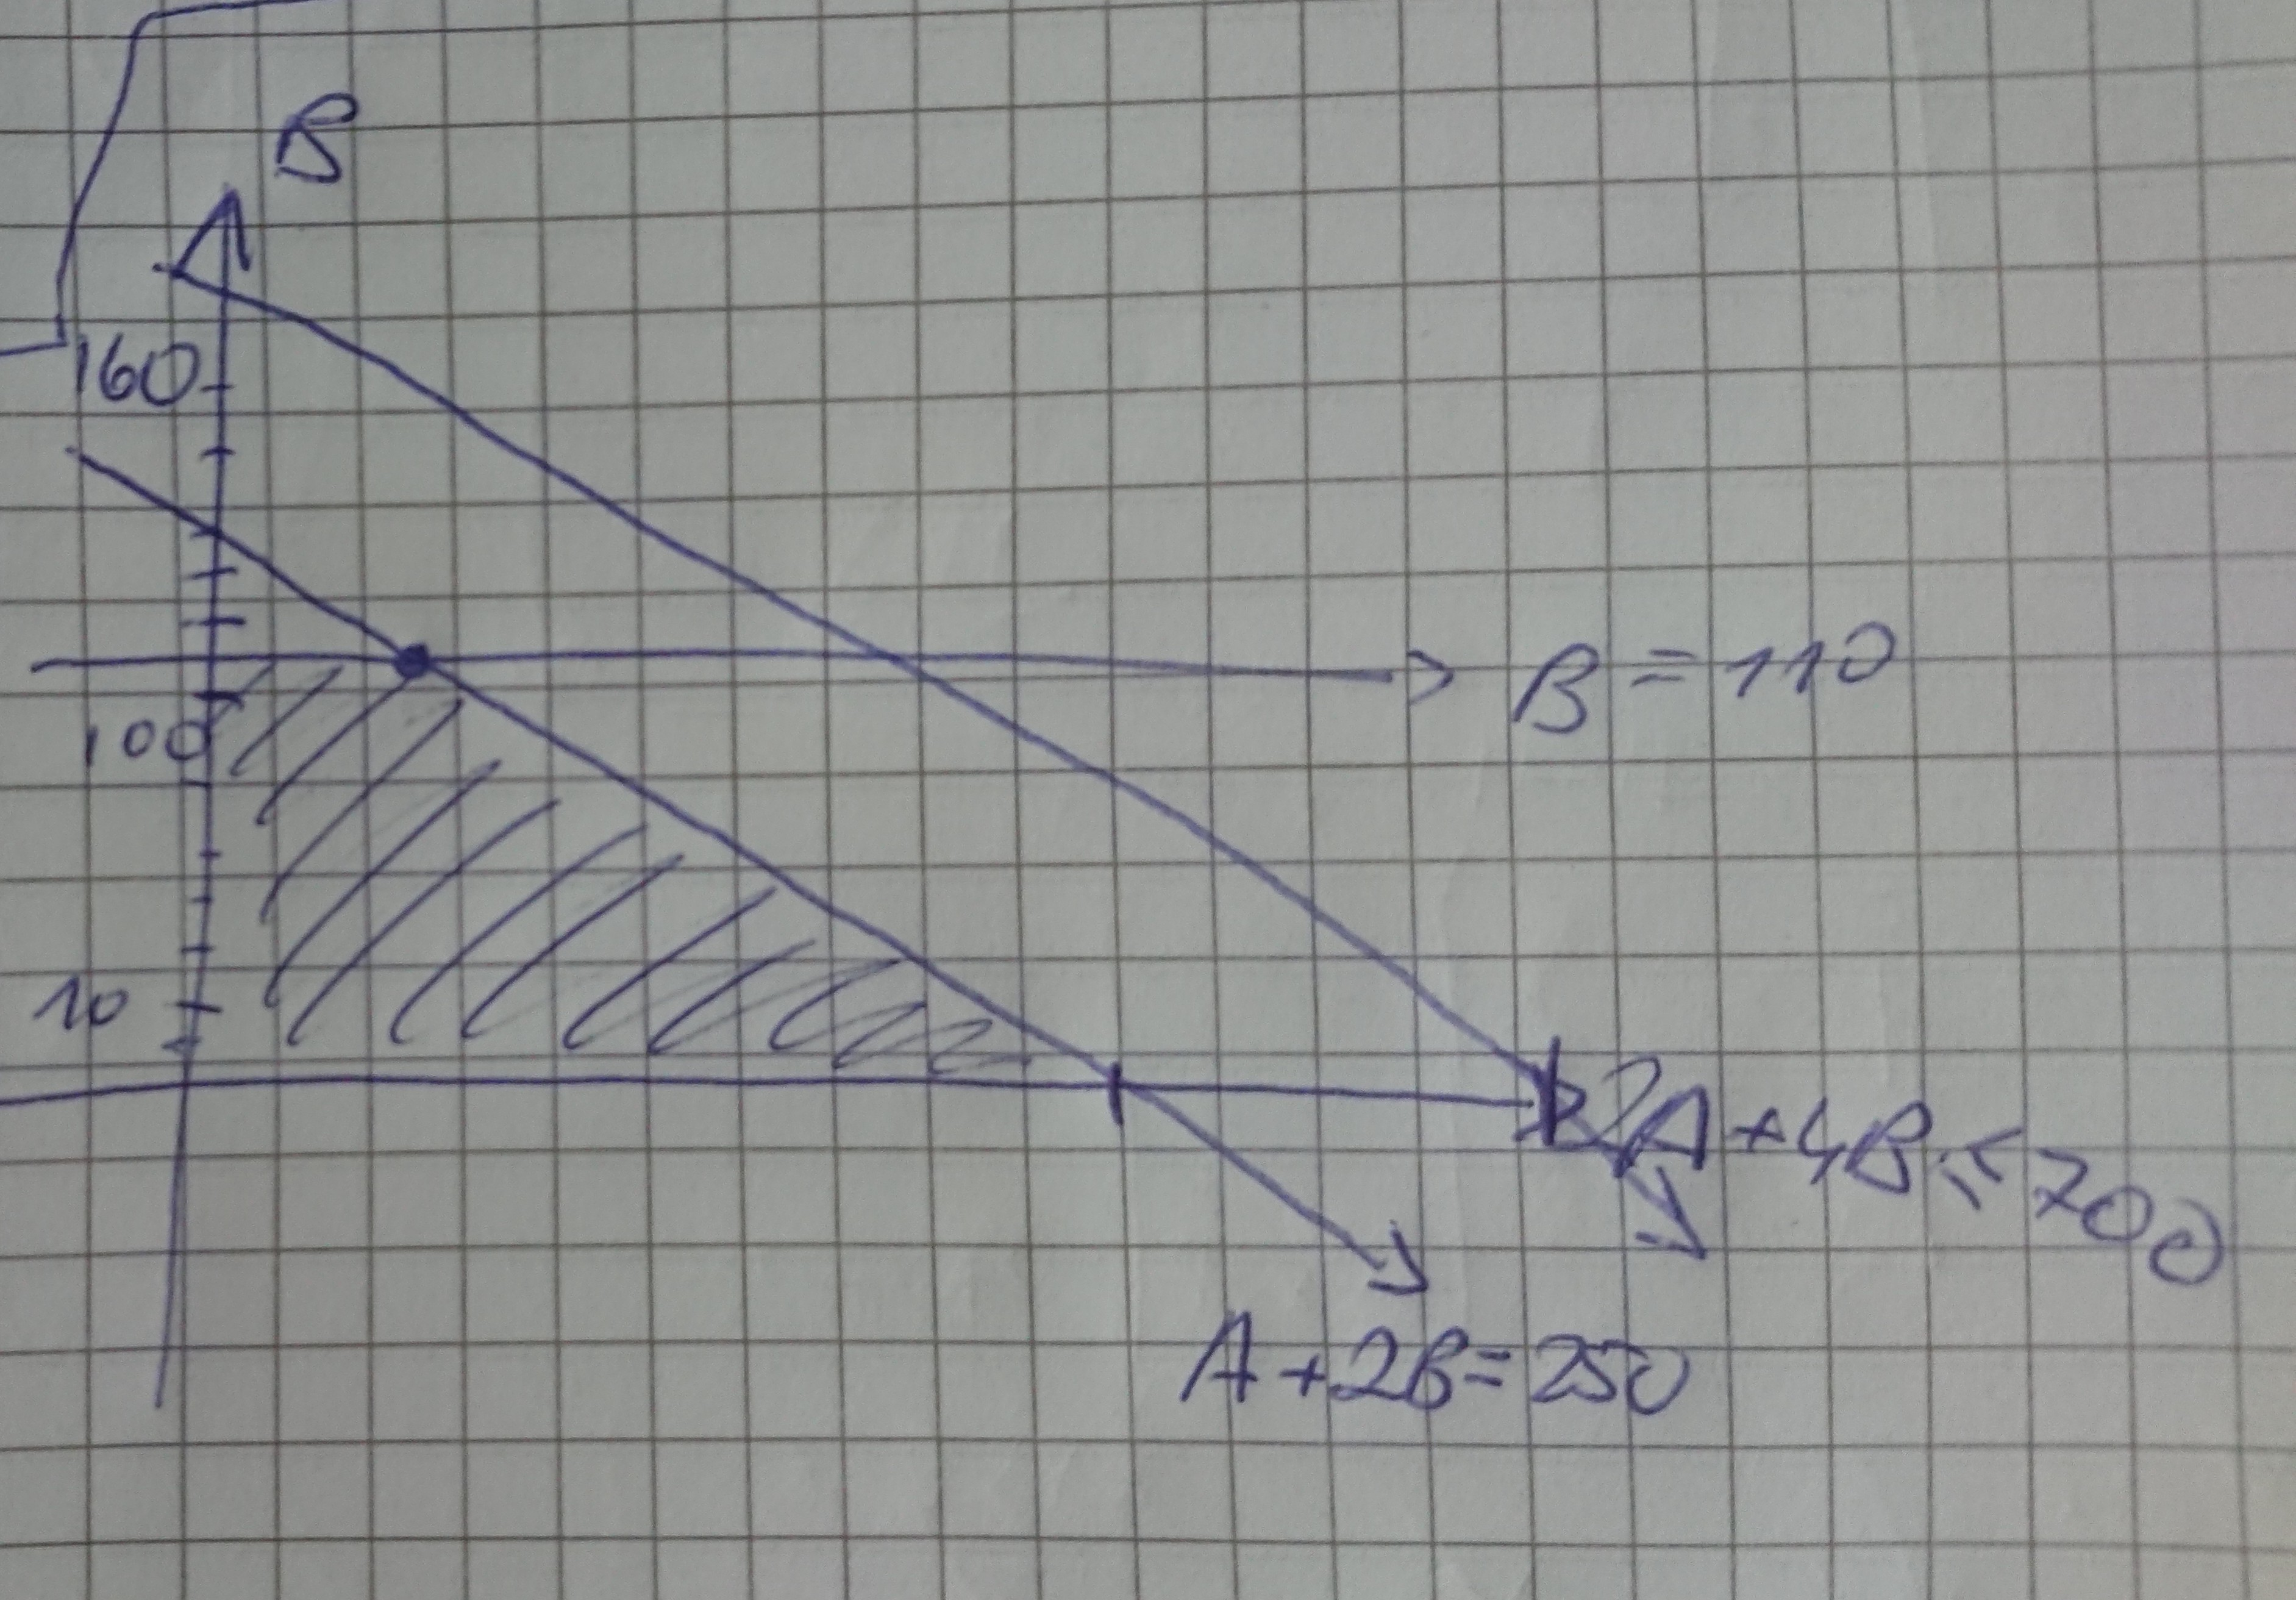
\includegraphics[width=6cm]{img/4_8_a}
	\end{figure}
	
	
	Rechnerisch: Wir möchten die Produktion von B maximieren sodass unsre Kapital größer wird. Also:\\
	
	Der limitierenden Bauteil für B ist die Spulen. Wir können maximal 110 Stück B bauen. Das heißt, wir brauchen auch 220 Kondensatoren, 440 Widerstände und 110 Spulen. Den Rest (im Lager bleibende): 30 Kondensatoren, 260 Widerstände. Das bedeutet, dass unsre limitierende Bauteil ist jetzt die Kondensatoren. Wir können zzgl. maximal 30 Stück A bauen. Unsre Gewinn lautet dann: 36000 Euros \\ 
	\item[b)] Wir müssen 150 Stück A Bauen. Nach der Einbau von A bleibt die Folgende im Lager: 100 Kondensatoren, 400 Widerstände und 110 Spulen. Wenn wir dann B bauen möchten, unsre limitierende Faktor dann ist Kondensatoren. Da wir 2 davon pro Stück B brauchen, können wir maximal 50 Stück B bauen. Also, unsre Gewinn ist: 30000 Euros\\
\end{itemize}

\end{document}